% !TeX spellcheck = pl_PL

\rozdzial

%%%%%%%%%%%%%%%%%%%%%%%%%%%%%%%%%%%%%%%%%%%%%%%%%%%%%%%%%%%%%%%%%%%%%%%
\section{Biuro}
\label{biuro}

W tym menu (rys. \ref{menuBiuro}) mamy możliwość przejścia między poszczególnymi modułami części biurowej, w skład której wchodzą:
\begin{itemize}
	\item \textbf{Zlecenie} - wszystkie operacje związane ze zleceniami (wprowadzanie, przegląd, edycja), zleceniodawcami (wprowadzanie, edycja) i meldunkami (przygotowanie, wydruk) - rozdz. \ref{zlecenie}.
	\item \textbf{Karta przyjęcia} - przegląd, edycja i wprowadzanie informacji dotyczących przyjęcia przyrządu, wprowadzanie nowych przyrządów, dodawanie sond - rozdz. \ref{karta_przyjecia}.
	\item \textbf{Cennik} - ustalanie cen wzorcowania danego przyrządu - rozdz. \ref{cennik}.
	\item \textbf{Rejestr zleceń} - przegląd wprowadzonych zleceń - rozdz. \ref{rejestr}.
\end{itemize}

Przycisk \textbf{"Zakończ"} cofa użytkownika do menu głównego (rys. \ref{menuGlowne}).

\begin{figure}[htb]
	\centering
	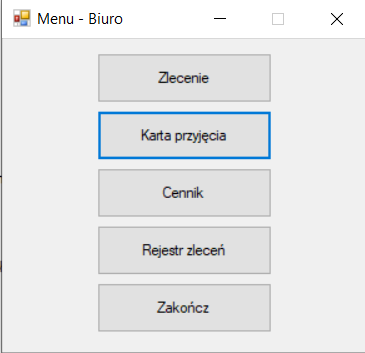
\includegraphics{obrazki/Biuro/menu_biuro.png}
	\caption{Menu części biurowej.}
	\label{menuBiuro}
\end{figure}

\subsection{Zlecenie}
\label{zlecenie}

W górnej części okna \textbf{"Zlecenie"} (rys. \ref{zlecenieDaneZleceniodawcy}) znajdują się ogólne informacje dotyczące zlecenia (niezależnie od wybranej zakładki) i przyciski pozwalające dodawać (\textbf{"Nowe zlecenie"}), usuwać (\textbf{"Usuń zlecenie"}) czy edytować zawartość zlecenia dodając do niego kolejne przyrządy (\textbf{"Dodaj kartę do zlecenia"}). 
W polu \textbf{"Numer zlecenia"} podany jest numer aktualnie przeglądanego zlecenia. Między poszczególnymi zleceniami można się poruszać za pomocą strzałek w tym polu, bądź też bezpośrednio wpisać wybrany przez nas numer zlecenia do pola. Jeżeli wchodzimy do Zlecenia z menu części biurowej, okno otwiera się automatycznie na ostatnim wprowadzonym zleceniu.
W polu \textbf{"Numer zlecenia w rejestrze"} należy wprowadzić numer tego zlecenia w "papierowym rejestrze zleceń". Ułatwi to poruszanie się pomiędzy obydwoma rejestrami.
 
 \begin{figure}[htb]
 	\centering
 	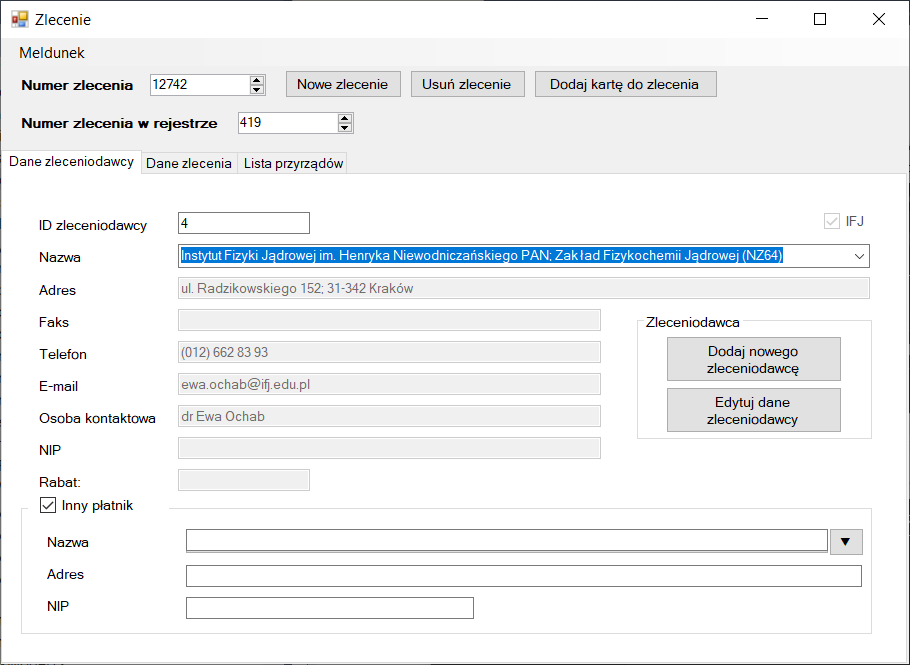
\includegraphics[width=\columnwidth]{obrazki/Biuro/zlecenie/zlecenie_dane_zleceniodawcy.png}
 	\caption{Zlecenie - zakładka z danymi zleceniodawcy.}
 	\label{zlecenieDaneZleceniodawcy}
 \end{figure}
 
Funkcje poszczególnych przycisków:
\begin{itemize}
	\item \textbf{Nowe zlecenie} - przejście do trybu dodawania nowego zlecenia. Wyświetli się okno z wyczyszczonymi polami. Nowemu zleceniu nadany będzie kolejny wolny numer zlecenia. Po wprowadzeniu odpowiednich danych należy zatwierdzić dodanie zlecenia przyciskiem \textbf{"Zatwierdź"}, który pojawił się w miejsce przycisku \textbf{"Nowe zlecenie"}. 
	\item \textbf{Usuń zlecenie} - przycisk usuwa aktualnie aktywne zlecenie. Jeżeli nie ma takiej konieczności, to nie zaleca się jego stosowania. Zamiast tego lepiej jest edytować błędne zlecenie wprowadzając poprawione dane tego, bądź nowego zlecenia.
	\item \textbf{Dodaj kartę do zlecenia} - przycisk uruchamia okno \textbf{"Karta przyjęcia"} (patrz rozdz. \ref{kartaDanePrzyrzadu}) pozwalając na przypisane wybranej karty przyjęcia do zlecenia.
\end{itemize}

	\textbf{TIP:} Mimo, iż aby dodać nowe zlecenie wystarczy podać jedynie zleceniodawcę (zakładka \textbf{"Dane zleceniodawcy"} - rys. \ref{zlecenieDaneZleceniodawcy}) warto jednak uzupełnić także zakładkę \textbf{"Dane zlecenia"} - rys. \ref{zlecenieDaneZlecenia}.

W lewym górnym rogu w rozwijanym menu \textbf{"Meldunek"} znajduje się przycisk umożliwiający podgląd w oknie przeglądarki internetowej i wydruk meldunku. Program umożliwi użycie tej opcji jedynie wtedy, kiedy zlecenie zostanie jako wykonane.

W zakładce \textbf{"Dane zleceniodawcy"} wprowadzamy dane zleceniodawcy. Należy rozpocząć od podania jego nazwy (pole \textbf{"Nazwa"}). Po wpisaniu pierwszych kilku liter na liście rozwijanej pojawią się pasujące propozycje nazw (użyta wielkość liter nie ma znaczenia). Jeżeli nazwa zleceniodawcy pojawiła się na liście należy ją wybrać. 

\textbf{WAŻNE:} Wprowadzając zleceniodawcę zawsze trzeba, jako zatwierdzenie wyboru, wybrać go z listy rozwijanej. Jeżeli operacja się powiodła, wtedy w pozostałych polach wyświetlą się wprowadzone wcześniej dane tego zleceniodawcy. Jeżeli dane się nie pojawią, oznacza to, że wybór zleceniodawcy został zakończony niepowiedzeniem.

\begin{figure}[htb]
	\centering
	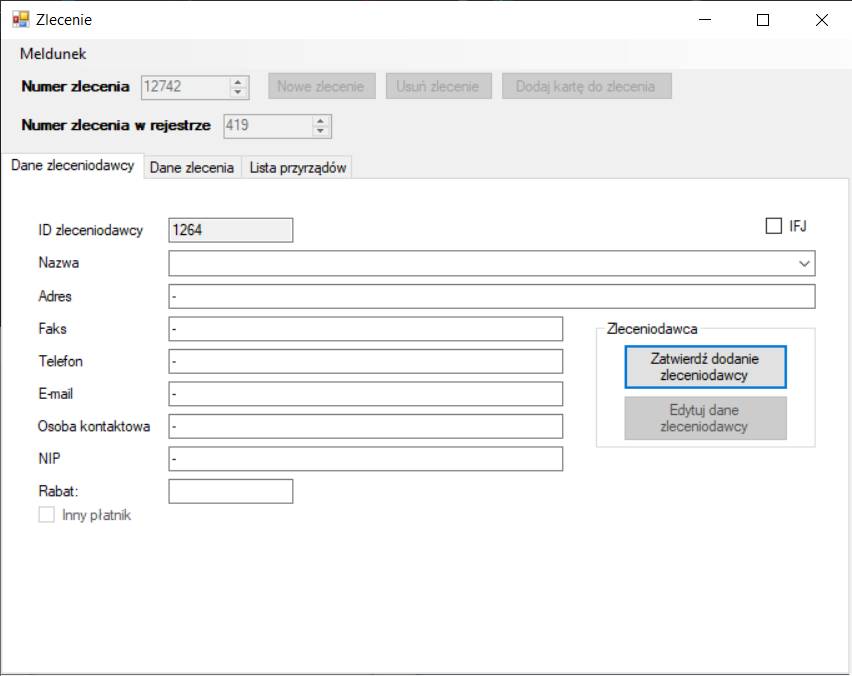
\includegraphics[width=\columnwidth]{obrazki/Biuro/zlecenie/zlecenie_dodanie_zleceniodawcy.png}
	\caption{Dodawanie nowego zleceniodawcy.}
	\label{zlecenieDodanieZleceniodawcy}
\end{figure}

\textbf{TIP:} Warto upewnić się, że znaleziony przez nas zleceniodawca jest tym, którego szukaliśmy sprawdzając pozostałe dane (przy okazji również sprawdzając ich aktualność). Jest to szczególnie ważne, w przypadku gdy jest szereg zleceniodawców o podobnej nazwie. Jeżeli dane nie są aktualne należy użyć przycisku \textbf{"Edytuj dane zleceniodawcy"}, wprowadzić poprawki, a następnie zatwierdzić je przyciskiem \textbf{"Zatwierdź"}, który pojawi się w miejsce przycisku \textbf{"Edytuj dane zleceniodawcy"}.

\textbf{TIP:} Można też wprowadzić zleceniodawcę wpisując jego numer ID w polu \textbf{"ID zleceniodawcy"}. Jest to zwiększająca wydajność metoda, szczególnie przydatna w~przypadku zleceniodawców często korzystających z usług Laboratorium Wzorcowania.

\textbf{TIP:} Pole \textbf{"Rabat"} podświetla się na czerwono, gdy jest wypełnione, po to aby zwrócić uwagę na przysługujący zleceniodawcy rabat.

Jeżeli nie znaleźliśmy zleceniodawcy w bazie danych należy wprowadzić go używając przycisku \textbf{"Dodaj nowego zleceniodawcę"} (rys. \ref{zlecenieDodanieZleceniodawcy}). W odpowiednie pola należy wprowadzić wszystkie posiadane dane: nazwa (pole \textbf{"Nazwa"}), adres (pole \textbf{"Adres"}), numer faksu (pole \textbf{"Faks"}), numer(y) telefonu (pole \textbf{"Telefon"}), adres e-mail (pole \textbf{"E-mail"}), dane osoby kontaktowej (pole \textbf{"Osoba kontaktowa"}), NIP (pole \textbf{"NIP"}), przysługujący rabat (pole \textbf{"Rabat"}) oraz oznaczenie czy zleceniodawca jest z Instytutu Fizyki Jądrowej PAN (pole wyboru  \textbf{"IFJ"}). ID zleceniodawcy zostanie nadane automatycznie. Po upewnieniu się, że wprowadzone dane są poprawne należy zatwierdzić za pomocą przycisku \textbf{"Zatwierdź dodanie zleceniodawcy"}, który pojawi się w miejsce przycisku \textbf{"Dodaj nowego zleceniodawcę"}.

\textbf{TIP:} Jedynie wprowadzenie nazwy zleceniodawcy jest obligatoryjne, jednak zaleca się podanie wszystkich posiadanych danych.

\textbf{TIP:} W nazwie zleceniodawcy i jego adresie, w miejscu gdzie na wydrukach (Świadectwie Wzorcowania, meldunku, karcie przyjęcia) chcemy uzyskać przejście do nowej linii należy wstawić średnik \textbf{";"}. 

\begin{figure}[htb]
	\centering
	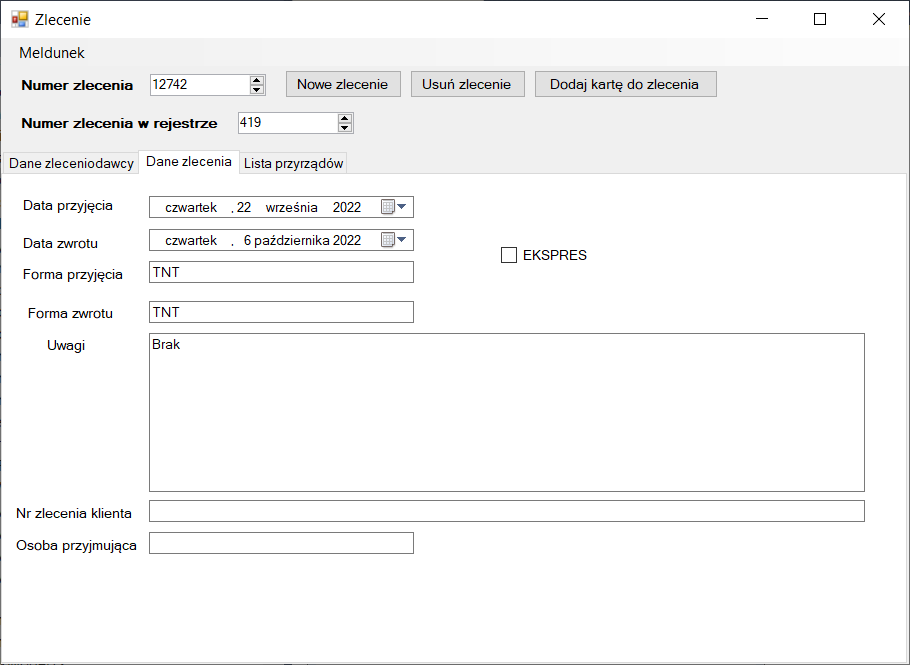
\includegraphics[width=\columnwidth]{obrazki/Biuro/zlecenie/zlecenie_dane_zlecenia.png}
	\caption{Zlecenie - zakładka z danymi zlecenia.}
	\label{zlecenieDaneZlecenia}
\end{figure}

Po wybraniu (lub wprowadzeniu) zleceniodawcy oraz uzupełnieniu pola \textbf{"Numer zlecenia w rejestrze"} możemy dodatkowo podać dane płatnika. Jest to opcja stosowana w przypadku, gdy zleceniodawca i płatnik nie sa tym samym podmiotem. W~tym celu należy zaznaczyć pole wyboru \textbf{"Inny płatnik"} (rys. \ref{zlecenieDaneZleceniodawcy}). Aktywuje to pola pozwalające na wprowadzenie danych płatnika. Jeżeli płatnik jest jednym ze zleceniodawców wprowadzonych wcześniej do bazy danych można wybrać jego nazwę z listy rozwijanej \textbf{"Nazwa"}. Po wpisaniu kilku liter lista ogranicza się do nazw zleceniodawców odpowiadających podanym literom (wielkość liter nie ma znaczenia). Po wybraniu nazwy pola \textbf{"Adres"} i \textbf{"NIP"} uzupełnią się automatycznie danymi z bazy. Jeżeli natomiast w~bazie danych nie ma danych płatnika można ręcznie wprowadzić je w odpowiednie pola (\textbf{"Nazwa"}, \textbf{"Adres"}, \textbf{"NIP"}). Dane te zostają przypisane tylko do tego zlecenia.

\textbf{TIP:} Jeżeli dany płatnik pojawia się regularnie warto wprowadzić jego dane do zleceniodawców, aby móc w przyszłości wyszukiwać je na liście rozwijanej, zamiast kolejny raz wprowadzać ręcznie.

\begin{figure}[htb]
	\centering
	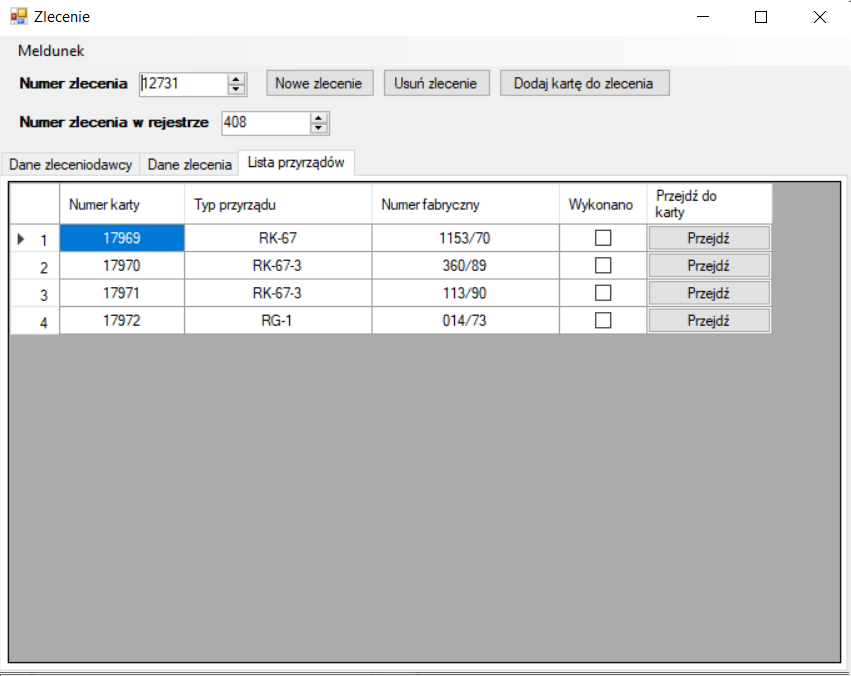
\includegraphics[width=\columnwidth]{obrazki/Biuro/zlecenie/zlecenie_lista.png}
	\caption{Zlecenie - zakładka z listą przyrządów przypisanych do zlecenia.}
	\label{zlecenieLista}
\end{figure}

W zakładce \textbf{"Dane zlecenia"} znajdują się różne dodatkowe informacje dotyczące zlecenia, takie jak: data przyjęcia zlecenia (\textbf{"Data przyjęcia"}), data jego zwrotu (\textbf{"Data zwrotu"}), forma przyjęcia przyrządów (\textbf{"Forma przyjęcia"}) i forma ich zwrotu (\textbf{"Forma zwrotu"}), numer zlecenia klienta (\textbf{"Nr zlecenia klienta"}), osoba przyjmująca zlecenie (\textbf{"Osoba przyjmująca"}) oraz dodatkowe uwagi (\textbf{"Uwagi"}). Tutaj także należy oznaczyć zlecenia, które mają być wykonane w trybie ekspresowym (pole wyboru \textbf{"Ekspres"}). 

\textbf{TIP:} Po wybraniu daty przyjęcia przyrządu, data zwrotu ustala się automatycznie na 14 dni po dacie przyjęcia. Jest to aktualnie ustalony maksymalny termin wykonania zlecenia. Jako formę zwrotu, przyjmuje się domyślnie, taką samą formę jak forma przyjęcia.

W zakładce \textbf{"Lista przyrządów"} wyświetla się tabela zawierająca informacje o~przyrządach, które mają być wywzorcowane w ramach danego zlecenia (rys. \ref{zlecenieLista}). Dla każdego z przypisanych do zlecenia przyrządów tabela podaje numer jego karty przyjęcia (kolumna \textbf{"Numer karty"}), typ i numer fabryczny (odpowiednio kolumny \textbf{"Typ przyrządu"} i \textbf{"Numer fabryczny"}) oraz informację czy wzorcowanie danego przyrządu zostało już wykonane (kolumna \textbf{"Wykonano"}). W ostatniej kolumnie znajduje się przycisk \textbf{"Przejdź"}, który otwiera okno z kartą przyjęcia tego przyrządu (patrz \ref{karta_przyjecia}).

\subsection{Karta przyjęcia}
\label{karta_przyjecia}

Do tej części programu można przejść albo bezpośrednio z menu części biurowej (rys. \ref{menuBiuro}), albo z zakładki \textbf{"Lista przyrządów"} w oknie \textbf{"Zlecenie"} (rys. \ref{zlecenieLista}) po użyciu przycisku \textbf{"Przejdź"}. W pierwszym przypadku okno otwiera się dla ostatniej wprowadzonej do bazy karty przyjęcia, w drugim dla karty, dla której został użyty przycisk. Trzecią opcją jest użycie przycisku \textbf{"Dodaj kartę do zlecenia"} z okna \textbf{"Zlecenie"} (patrz rozdz. \ref{zlecenie}). Tutaj uruchamia się pusta karta przyjęcia.

W górnej części okna \textbf{"Karta przyjęcia"} znajdują się pola z numerem karty (\textbf{"Numer karty"}), numerem zlecenia, do którego przypisana jest ta karta (\textbf{"Numer zlecenia"}) oraz rokiem, w którym dana karta została wprowadzona do bazy danych (\textbf{"Rok"}).
Poniżej znajdują się pola wyboru: \textbf{"Wykonano"} oraz \textbf{"Uszkodzony"}. Pierwsze należy zaznaczyć, kiedy zakończono już wzorcowanie przyrządu i wystawiono Świadectwo Wzorcowania. Drugi natomiast służy do oznaczania przyrządów uszkodzonych, których wzorcowanie, a co za tym idzie wystawienie Świadectwa Wzorcowania, nie było możliwe.

Po prawej znajdują się przyciski:
\begin{itemize}
	\item \textbf{"Cennik"} - otwiera okno cennika (patrz rozdz. \ref{cennik}). W oknie tym zaznaczone zostały podstawowe wymagania dotyczące kalibracji. Program przyjmuje domyślnie podstawowe formy wzorcowania, więc wszelkie zmiany jak np. inny wariant wzorcowania w zakresie mocy dawki, czy zwiększona liczba progów w~sygnalizacji, należy wprowadzić ręcznie.
	\item \textbf{"Wzorcuj"} - przejście do głównego okna wzorcowania dla tego numeru karty przyjęcia.
\end{itemize}

\begin{figure}[htb]
	\centering
	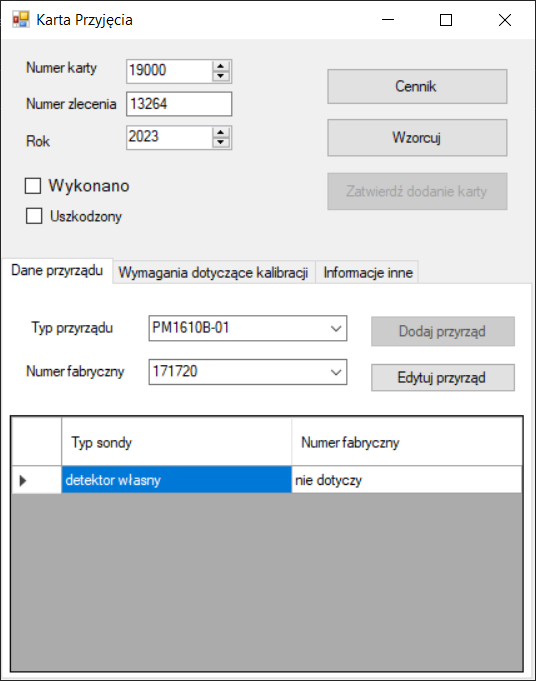
\includegraphics{obrazki/Biuro/karta/karta_dane_przyrzadu.png}
	\caption{Karta przyjęcia - zakładka z danymi przyrządu.}
	\label{kartaDanePrzyrzadu}
\end{figure}

W zakładce \textbf{"Dane przyrządu"} wprowadza się dane przyrządu (rys. \ref{kartaDanePrzyrzadu}). Najpierw należy wprowadzić typ (pole \textbf{"Typ przyrządu"}). Po wpisaniu kilku liter można wybrać go z listy rozwijanej (wielkość stosowanych liter nie ma znaczenia). Po wybraniu typu należy wprowadzić i wybrać z listy rozwijanej (pole \textbf{"Numer fabryczny"}) numer fabryczny przyrządu znajdujący się na jego tabliczce znamionowej. Poniżej w tabeli powinna pokazać się lista sond przypisanych do tego przyrządu (typ - kolumna \textbf{"Typ przyrządu"} i numer fabryczny - kolumna \textbf{"Numer fabryczny"}). W~przypadku, gdy przyrząd ma tylko wbudowany detektor, wyświetli się "detektor własny" jako typ sondy i "nie dotyczy" jako jej numer fabryczny. 

\textbf{WAŻNE:} Wprowadzając typ i numer fabryczny przyrządu do karty przyjęcia trzeba, jako zatwierdzenie wyboru, wybrać go z listy rozwijanej. Jeżeli w tabeli nie wyświetli się żadna sonda oznacza to, że wprowadzanie danych przyrządu z jakiejś przyczyny nie powiodło się.

Jeżeli w bazie nie ma danego numeru fabrycznego lub (co rzadsze) nie ma danego typu przyrządu należy go wprowadzić klikając przycisk \textbf{"Dodaj przyrząd"}. Otworzy się okno umożliwiające wprowadzenie danych nowego przyrządu (rys. \ref{edytujPrzyrzad}). ID przyrządu  (pole \textbf{"ID przyrządu"}) ustalane jest przez program automatycznie. Użytkownik powinien podać typ (pole \textbf{"Typ"}) i numer fabryczny (pole \textbf{"Numer fabryczny"}) sczytane z tabliczki znamionowej przyrządu, rok produkcji (pole \textbf{"Rok produkcji"}), producenta (pole \textbf{"Producent"}) oraz nazwę przyrządu (pole \textbf{"Nazwa"}) np. radiometr, monitor skażeń, dawkomierz, etc.

\textbf{TIP:} Wszystkie powyższe informacje można zazwyczaj znaleźć na tabliczce znamionowej lub w instrukcji obsługi przyrządu. Część z nich jest często również dostępna na stronie producenta.

\begin{figure}[htb]
	\centering
	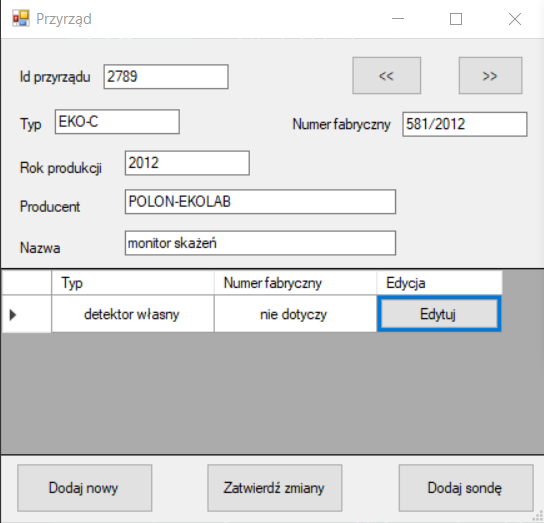
\includegraphics{obrazki/Biuro/karta/edytuj_przyrzad.png}
	\caption{Okno edycji danych przyrządu.}
	\label{edytujPrzyrzad}
\end{figure}

\begin{figure}[htb]
	\centering
	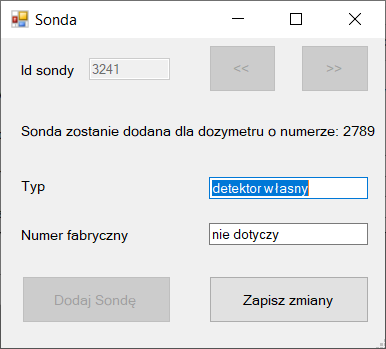
\includegraphics{obrazki/Biuro/karta/edytuj_sonde.png}
	\caption{Okno edycji sondy.}
	\label{edytujSonde}
\end{figure}

Kolejno należy podać wszystkie sondy przyrządu. W tym celu używamy przycisku \textbf{"Dodaj sondę"}, która otwiera nowe okno - \textbf{"Sonda"} (rys. \ref{edytujSonde}). W przypadku sondy podajemy tylko jej typ (pole \textbf{"Typ"}) i numer fabryczny (pole \textbf{"Numer fabryczny"}) umieszczone na jej tabliczce znamionowej.

\textbf{TIP:} Jeżeli przyrząd posiada wyłącznie wbudowany detektor bez osobnego numeru fabrycznego w polu \textbf{"Typ"} należy podać "detektor własny", a w polu \textbf{"Numer fabryczny"} - "nie dotyczy". 

Po wprowadzeniu sondy należy zatwierdzić przyciskiem \textbf{"Zapisz zmiany"}. 

\begin{figure}[htb]
	\centering
	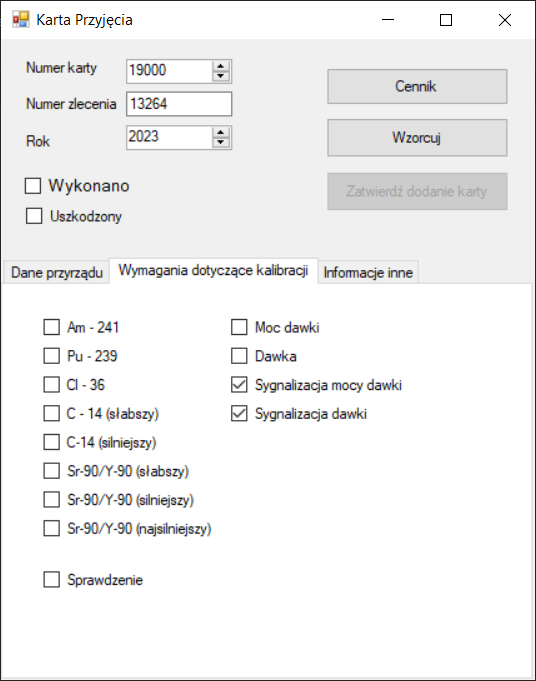
\includegraphics{obrazki/Biuro/karta/karta_dane_wymagania.png}
	\caption{Karta przyjęcia - zakładka z informacjami o danych dotyczących kalibracji.}
	\label{kartaDaneKalibracji}
\end{figure}

\textbf{TIP:} Zaleca się takie wprowadzanie danych, aby poszczególne sondy dozymetru były łatwo rozróżnialne.

W tabeli w oknie \textbf{"Przyrząd"} (rys. \ref{edytujPrzyrzad}), w ostatniej kolumnie, przy każdej z sond znajduje się przycisk \textbf{"Edytuj"}, który przechodzi do analogicznego okna \textbf{"Sonda"} (rys.~\ref{edytujSonde}), w którym można edytować dane już istniejących w bazie sond. 

Okno \textbf{"Przyrząd"} (rys. \ref{edytujPrzyrzad}) uruchamia się także w przypadku edycji przyrządu, do której można przejść za pomocą przycisku \textbf{"Edytuj przyrząd"} w zakładce \textbf{"Dane przyrządu"} (rys. \ref{kartaDanePrzyrzadu}). Każdorazowo po wprowadzeniu zmian należy pamiętać o ich zatwierdzeniu przyciskiem \textbf{"Zatwierdź zmiany"}.
 
 \begin{figure}[htb]
 	\centering
 	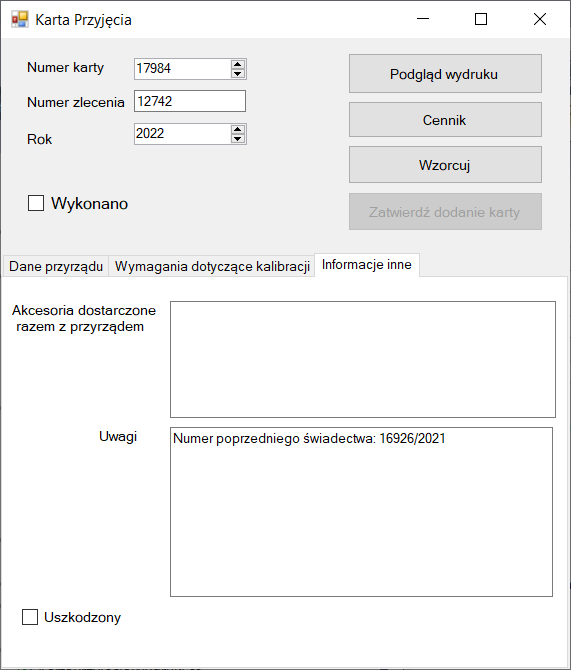
\includegraphics{obrazki/Biuro/karta/karta_dane_inne.png}
 	\caption{Karta przyjęcia - zakładka z pozostałymi danymi.}
 	\label{kartaDaneInne}
 \end{figure}

W zakładce \textbf{"Wymagania dotyczące kalibracji"} znajdują się informacje odnośnie tego jaki jest zakres wzorcowania danego przyrządu. Można wybrać jeden z~czterech rodzajów wzorcowania promieniowaniem gamma (moc dawki, dawka, sygnalizacja i sygnalizacja mocy dawki) oraz dowolne z ośmiu źródeł stosowanych do wzorcowania w zakresie emisji powierzchniowej. W przypadku promieniowania alfa są to Am-241 oraz Pu-239, a w przypadku promieniowania beta mamy do dyspozycji, dwa źródła C-14 o różnej wartości emisji powierzchniowej, trzy źródła Sr-90/Y-90 o różnej wartości emisji powierzchniowej oraz Cl-36. 

Jest też dostępna opcja \textbf{"Sprawdzenie"}. Zaznaczenie tej opcji spowoduje odznaczenie wszystkich innych.

Podany w karcie przyjęcia zakres wzorcowania jest stosowany automatycznym wyliczeniu ceny wzorcowania dla tej karty (patrz \ref{cennik}) oraz odblokowuje odpowiednie przyciski w głównym oknie wzorcowania (patrz \ref{wzorcowanie}).

Zakładka \textbf{"Informacje inne"} zawiera pola umożliwiające wprowadzenie dodatkowych informacji związanych z danym przyrządem (pola \textbf{"Akcesoria dostarczone razem z przyrządem"} oraz \textbf{"Uwagi"}). Jeżeli przyrząd był wcześniej wzorcowany w Laboratorium Wzorcowania, to w polu \textbf{"Uwagi"} automatycznie uzupełnia się numer poprzedniego świadectwa wzorcowania wystawionego dla tego przyrządu.

\subsection{Cennik}
\label{cennik}

W tej części (rys. \ref{cennikRys}) można ręcznie ustalić cenę usługi dla klienta w zależności od wybranego przez niego zakresu wzorcowania i typu przyrządu. Można do niej przejść bezpośrednio z karty przyjęcia (patrz rozdz. \ref{karta_przyjecia}) lub z menu głównego części biurowej (rys. \ref{menuBiuro}). W pierwszym przypadku pola w cenniku są wstępnie uzupełnione danymi z karty przyjęcia z zakładki \textbf{"Wymagania dotyczące kalibracji"} (rys. \ref{kartaDaneKalibracji}). W drugim otwiera się puste okno cennika, które można dowolnie wypełniać.

W pierwszej kolejności należy wypełnić część \textbf{"Rodzaje wzorcowań"} wprowadzając liczbę poszczególnych typów wzorcowań (mocy dawki, dawki, emisji powierzchniowej i~sygnalizacji). W zależności od wybranych w tej części okna opcji, odblokuje się możliwość podania bardziej szczegółowych parametrów, dla poszczególnych typów wzorcowań.

\textbf{Ważne:} Pod terminem \textbf{"Sygnalizacja"} mieści się zarówno wzorcowanie w zakresie sygnalizacji dawki jak i sygnalizacji mocy dawki.

Jeżeli wybrana została opcja mocy dawki należy podać odpowiedni wariant wzorcowania zaznaczając odpowiednio:
\begin{itemize}
	\item \textbf{Podstawowy} - wszystkie standardowe wzorcowania;
	\item \textbf{Rozszerzony} - rozszerzone wzorcowania (wzorcowania w szerszym zakresie wartości wzorcowych, z większą ilością punktów pomiarowych);
	\item \textbf{Trudny} - wzorcowania, które z jakiegoś powodu są trudniejsze do wykonania, albo zajmują dużo więcej czasu (np. duże gabaryty przyrządu, długi czas ustalania wskazań przyrządu).
\end{itemize}

\textbf{TIP:} Jeżeli okno cennik otwarte zostanie dla karty przyjęcia, dla której wzorcowanie w zakresie mocy dawki zostało już wykonane, to program zasugeruje użytkownikowi, jeżeli wykryje, że wzorcowanie jest najprawdopodobniej w rozszerzonym zakresie. Obok pola wyboru wariantu mocy dawki pojawi się na czerwono komunikat: "Najprawdopodobniej jest to rozszerzone wzorcowanie"

\begin{figure}[htb]
	\centering
	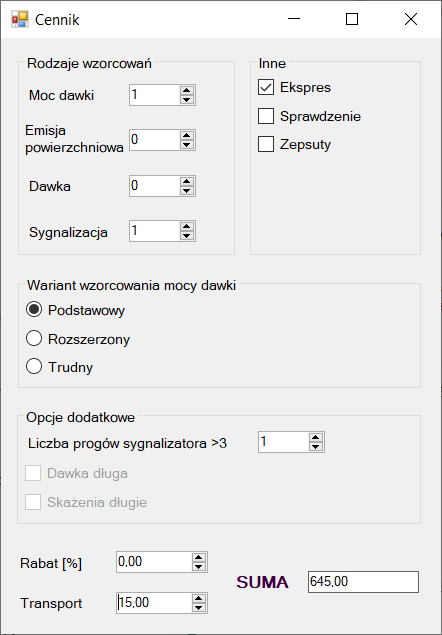
\includegraphics{obrazki/Biuro/cennik.png}
	\caption{Okno cennika}
	\label{cennikRys}
\end{figure}

W szczególnych przypadkach możliwe jest zaznaczenie opcji dodatkowych (część \textbf{"Opcje dodatkowe"}):
\begin{itemize}
	\item \textbf{Liczba progów sygnalizatora $>$ 3} - należy podać jaka liczba progów (ponad podstawowe 3) została wywzorcowana;
	\item \textbf{Dawka długa} - w przypadku przyrządów, dla których wzorcowanie w zakresie dawki trwa dłużej niż standardowo (np. przyrząd można naświetlać jedynie z niską mocą dawki);
	\item \textbf{Skażenia długie} - dłuższe i bardziej pracochłonne wzorcowanie w zakresie emisji powierzchniowej.
\end{itemize}

W części \textbf{"Inne"} można zaznaczyć:
\begin{itemize}
	\item \textbf{Ekspres} - jeżeli wzorcowanie ma zostać wykonane w trybie ekspresowym;
	\item \textbf{Sprawdzenie} - jeżeli przyrząd nie podlega standardowemu wzorcowaniu zakończonemu wystawieniem świadectwa, a jedynie sprawdzeniu czy działa (w~jednym punkcie pomiarowym);
	\item \textbf{Zepsuty} - jeżeli przyrząd jest uszkodzony i niezdatny do wzorcowania.
\end{itemize}

Dodatkowo jest możliwość podania rabatu przysługującego danemu zleceniodawcy na to zlecenie (pole \textbf{"Rabat}) (rabat podajemy w procentach) oraz doliczenie kosztów transportu. W przypadku gdy jego koszt ma ponieść Laboratorium Wzorcowania (pole \textbf{"Transport"}).

Wynik podawany jest w złotówkach w polu \textbf{"Suma"}.

\textbf{TIP:} Wszystkie podstawowe ceny przechowywane są w pliku MS Access bazy danych w tabeli \textbf{"Cennik"}. 


\subsection{Rejestr zleceń}
\label{rejestr}

Rejestr zleceń (rys. \ref{rejestrZlecen}) służy do przeglądania wprowadzonych do bazy zleceń. 

Zawiera on zestawienie następujących informacji: 
\begin{itemize}
	\item numer zlecenia - kolumna \textbf{"Nr zlecenia"};
	\item nazwa zleceniodawcy - kolumna \textbf{"Zleceniodawca"};
	\item data przyjęcia - kolumna \textbf{"Data przyjęcia"};
	\item forma przyjęcia - kolumna \textbf{"Forma przyjęcia"};
	\item data zwrotu - kolumna \textbf{"Data zwrotu"};
	\item forma zwrotu - kolumna \textbf{"Forma zwrotu"};
	\item planowany termin wykonania - kolumna \textbf{"Planowany termin wykonania"};
	\item czy zlecenie zostało wykonane - kolumna \textbf{"Wykonano"};
	\item całkowita liczba przyrządów w zleceniu - kolumna \textbf{"Liczba przyrządów w~zleceniu"};
	\item liczba przyrządów przed wzorcowaniem - kolumna \textbf{"Liczba przyrządów przed wzorcowaniem"};
	\item lista przyrządów pogrupowanych ze względu na typ - kolumna \textbf{"Lista przyrządów"};
\end{itemize}

Rejestr można wyświetlić dla danego miesiąca wprowadzając wybrany miesiąc (pole \textbf{"Miesiąc"}) i rok (pole \textbf{"Rok"}). 

\textbf{TIP:} Korzystając z rejestru zleceń można w prosty sposób przejrzeć listę aktualnych zleceń i wydajnie zaplanować pracę np. łącząc kalibracje tych samych typów przyrządów w jeden blok, co pozwala uniknąć wielokrotnego pozycjonowania przyrządów tego samego typu.

\begin{sidewaysfigure}[p]
	\centering
	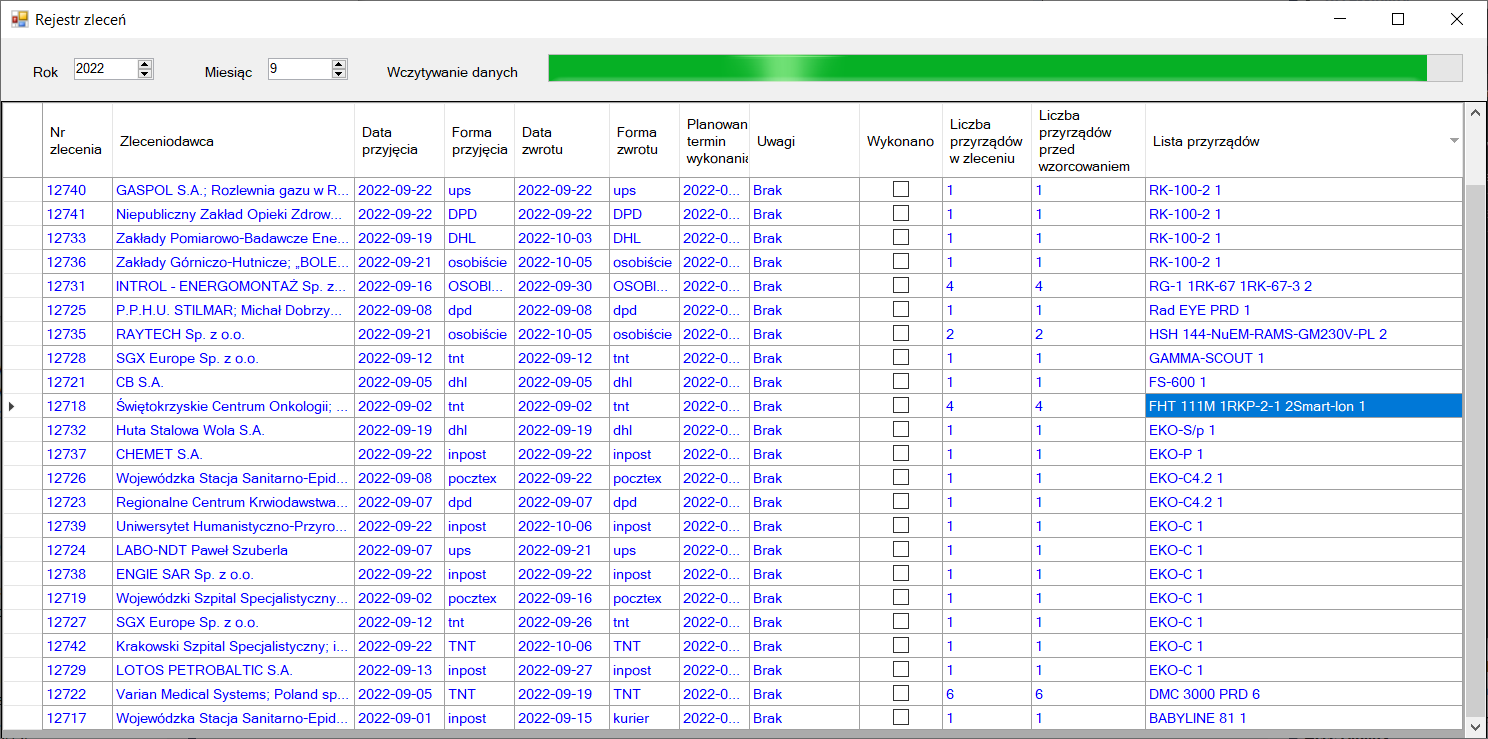
\includegraphics[width=\columnwidth]{obrazki/Biuro/rejestr_zlecen.png}
	\caption{Rejestr zleceń}
	\label{rejestrZlecen}
\end{sidewaysfigure}